\section{Dataset Preparation}

\subsection{Source Separation}

Following the selection of the two albums for each artist and removal of any songs where additional vocal artists to the main vocalist featured were removed, all songs were passed through the pre-trained Spleeter model\cite{SpleeterPip}\cite{SpleeterPip}. This pre-trained model can carry out source separation of instrumental and music tracks. Source separation was essential as the training dataset must not contain any instrumentals. The model outputted two separate tracks for each song, one representing the instrumentals and one the vocals. The instrumental tracks were discarded.

Using Spleeter to split existing songs with instrumental components opened up the possibility of using a more significant number of songs, something the original singing DDPS paper's authors did not consider. Their largest single voice dataset had a compressed size of ~70Mb, whereas the pre-processed datasets used in this thesis were approximately ten times that at ~700Mb, whilst still being based on a single vocal artist, style of music, and vocals only tracks. Using a more extensive training dataset would reduce over-fitting and aid generalisation. The remaining vocal tracks were then pre-processed.

\subsection{Pre-processing}

\begin{figure}[H]
    \centering
    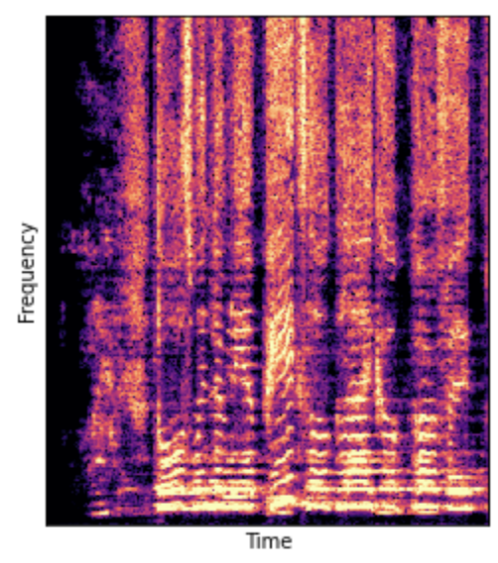
\includegraphics[width=0.6\textwidth]{research/dataset_preparation/PreprocessingSpecplot.png}
    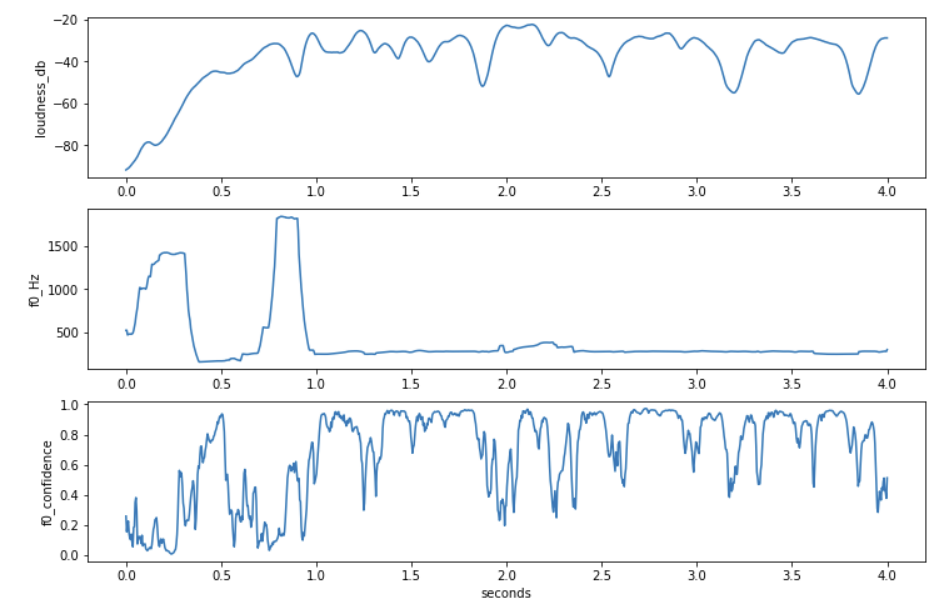
\includegraphics[width=0.8\textwidth]{research/dataset_preparation/PreprocessingFeatures.png}
    \caption{Dataset Pre-processing: Spectrogram plot of a random 4 second sample from one of the datasets and its accomanying F0, F0 Confidence and Amplitude characteristics over time throughout the sample}
\end{figure}

Pre-processing the datasets involved splitting the raw audio into smaller frames (samples), each 4 seconds long. The frame length was limited to 4 seconds to avoid capturing too much information in one spectrogram, which would make learning using the convolutional neural network difficult.

For each frame, F0 and confidence of F0 probability were inferred using CREPE\cite{CREPE}. Amplitude was computed statistically using the Librosa library\cite{LibrosaPip}. Latent Z information was available by passing the raw audio through the encoder. The 4-second samples and accompanying features were then stored as TFRecord files.

Each of the two datasets was pre-processed on Google Colab notebooks; this process took approximately 40 minutes for each dataset using an NVIDIA Tesla V100 GPU.

Finally, a random 4-second clip was selected from each dataset to prove successful pre-processing. Its spectrogram was computed and plotted. Computed F0, F0 Confidence and Amplitude characteristics were also plotted for the selected clip. The underlying audio sample could also be played.